Lato view ho implementato la mappa di gioco, con il supporto di Meshua Galassi e Lorenzo Chiana. 
La mappa di gioco, rappresentata dalla case class \textit{FXGameScene}, viene aggiornata dal \textit{GameManager} ad ogni step. Mantiene una serie di \textit{Map} che rappresentano i vari elementi che devono essere disegnati e spostati ad ogni step. La collezione mappa l'id dell'elemento alla propria \textit{ImageView}. Ad ogni update si controlla se gli elementi hanno subito variazioni dall'update precedente, in caso affermativo vengono ridisegnate nella posizione corretta o eliminate.
Mantenendo questa serie di \textit{Map} si evita di svuotare e ripopolare l'arena di gioco ad ogni step. In questo modo non si rischia di sovraccaricare il \textit{JavaFX Application Thread}.

Inizialmente \textit{FXGameScene} conteneva la gestione di tutti gli elementi da visualizzare. Successivamente si è scelto di rifattorizzarla per renderla meno prolissa, più organizzata e più leggibile. 
Durante la rifattorizzazione sono state create le seguenti case class di supporto:

\begin{itemize}
    \item \textbf{ArenaRoom}
    \item \textbf{Bullets}
    \item \textbf{Collectibles}
    \item \textbf{Enemies}
    \item \textbf{Player}
\end{itemize}

\begin{figure}[H]
\centering
  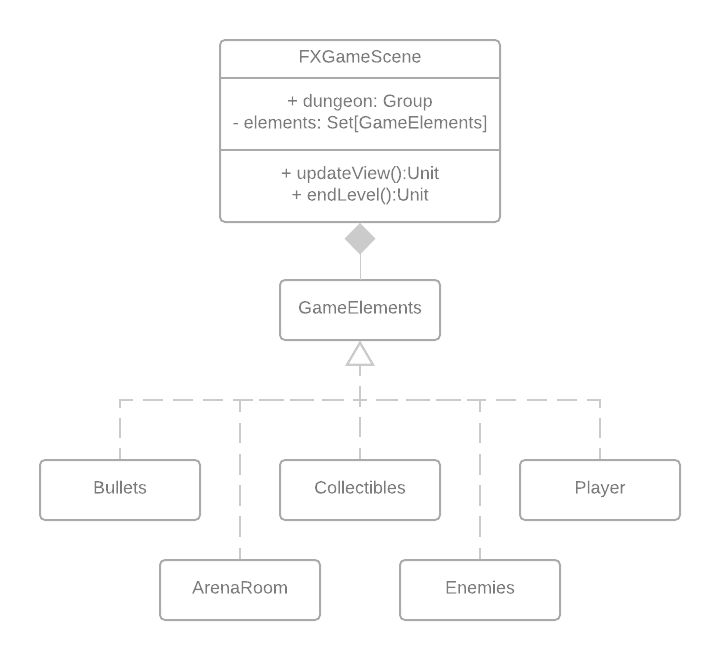
\includegraphics[width=11cm]{res/VIEW_Diagram.png}
  \caption{Organizzazione dell'arena di gioco}
  \label{view}
\end{figure}

Come si evince dalla figura \ref{view}, tutte estendono dalla trait \textit{GameElements}, che vuole rappresentare genericamente qualsiasi elemento che deve essere disegnato e aggiornato nell'arena di gioco. L'object \textit{GameElements} fornisce metodi di util, utili per i vari elements come riportato in figura \ref{gameElements}

\begin{figure}[H]
\centering
  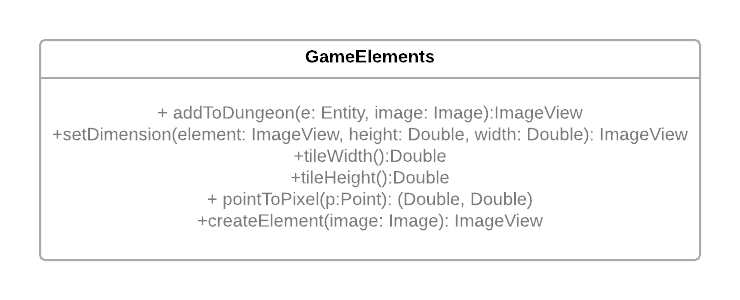
\includegraphics[width=14cm]{res/gameElements_Diagram.png}
  \caption{Metodi util di GameElements}
  \label{gameElements}
\end{figure}
